%-------------------------------------------------------------------------------
\section{Einführung in die Vorlesung}
%-------------------------------------------------------------------------------

%%% Folie
{
\scriptsize

\begin{frame}{Inhalte der Vorlesung}
    \begin{columns}
        \begin{column}[T]{.7\textwidth}
            \begin{block}{Übergeordnete Lernziele}
                \begin{itemize}
                    \item Die vorhandenen Programmierkenntnisse praktisch anwenden können
                    \item Eingebettete IoT-Anwendungen in Python programmieren können
                    \item Für IoT-Anwendungen nützliche Python-Bibliotheken nutzen können
                    \item Nach Bibliotheken suchen und sich in diese einarbeiten können
                \end{itemize}
            \end{block}

            \begin{block}{Themenschwerpunkte}
                \begin{itemize}
                    %~ \item Definition und Architektur des Internet of Things
                    %~ \item Ansteuerung von Hardwarebausteinen über den GPIO-Port
                    %~ \item Datenaustausch in verteilten IoT-Systemen
                    %~ \item Ablage von Messwerten und Sensordaten in einer Datenbank
                    %~ \item Visualisierung und Auswertung der gespeicherten Sensordaten
                    \item Grundlagen des Internet of Things
                    \item Hardwarenahe Programmierung in Python
                    \item Datenauschtausch in verteilten IoT-Systemen
                    \item Messwerte und Sensordaten speichern
                    \item Daten visualisieren und auswerten
                \end{itemize}
            \end{block}
        \end{column}

        \begin{column}[T]{.3\textwidth}
            \includegraphics[width=\textwidth]{img/depressed-developer-35}
        \end{column}
    \end{columns}
\end{frame}
}

{
\footnotesize

%%% Folie
\begin{frame}{Didaktisches Modell}
    \begin{columns}
        \begin{column}[T]{.5\textwidth}
            \textbf{Ablauf der Vorlesungsstunden}
            \medskip

            \begin{enumerate}
                \item Fragen und Wiederholung
                \item Besprechung des jeweiligen Themas
                \item Entwicklung eines Fallbeispiels
            \end{enumerate}
        \end{column}

        \begin{column}[T]{.5\textwidth}
            \textbf{Prüfungsleistung}
            \medskip

            \Justified{
                Praktische Assigment-Aufgabe basierend auf den in der
                Vorlesung behandelten Fallbeispielen.
            }
        \end{column}
    \end{columns}

    \vfill

    \begin{columns}
        \begin{column}[T]{.5\textwidth}
            \includegraphics[width=\textwidth]{img/linus-torvalds-house}
        \end{column}
        \begin{column}[T]{.5\textwidth}
            \includegraphics[width=\textwidth]{img/ghost-in-the-shell}
        \end{column}
    \end{columns}
\end{frame}
}

%%% Folie
{
\footnotesize

\begin{frame}{Benötigte Hard- und Software}
        \begin{columns}
            \begin{column}[T]{.5\textwidth}
                \textbf{Hardware}
                \medskip

                \Justified{
                    \scriptsize
                    Vor über einem Jahr wurden 30 neue Rasbperry Pi bestellt, die wegen
                    der weltweiten Materialengpässe immer noch nicht geliefert wurden \ldots
                    Da wir deshalb keine reale Hardware zur Verfügung haben, werden wir
                    diese in der Vorlesung mit Python simulieren. \smiley{}
                }
                \medskip

                \begin{itemize}
                    \item \textcolor{darkgray}{Raspberry Pi}
                    \item \textcolor{darkgray}{Diverse Sensoren und Aktoren}
                \end{itemize}
            \end{column}
            \begin{column}[T]{.5\textwidth}
                \textbf{Software}
                \medskip

                \Justified{
                    \scriptsize
                    Im einfachsten Fall benötigen Sie gar nichts, außer einem GitHub-Benutzer.
                    Die unten aufgeführten Tools können dann mit Gitpod online ausgeführt werden.
                    Gitpod stellt hierfür eine Online-IDE basierend auf Visual Studio Code und
                    eine fertig konfigurierte Linux-VM zur Verfügung.
                }
                \medskip

                \begin{itemize}
                    \item Visual Studio Code
                    \item Python
                    \item Docker
                    \item Git
                \end{itemize}
            \end{column}
        \end{columns}
\end{frame}
}

%%% Folie
{
\footnotesize
\setlength{\fboxsep}{0pt}

\begin{frame}{Literaturempfehlungen}
    \fbox{\includegraphics[height=3.3cm]{img/buch_raspberrypi}}
    \hfill
    \fbox{\includegraphics[height=3.3cm]{img/buch_python3_handbuch}}
    \hfill
    \fbox{\includegraphics[height=3.3cm]{img/buch_practical_electronics}}
    \hfill
    \fbox{\includegraphics[height=3.3cm]{img/buch_embedded_hardware}}

    \vskip 0.6cm

    \begin{columns}
        \column[T]{.5\textwidth}
        \textbf{Raspberry Pi: Das umfassende Handbuch} \\ Rheinwerk Verlag, 2018

        \column[T]{.5\textwidth}
        \textbf{Python 3: Das umfassende Handbuch} \\ Rheinwerk Verlag, 2023
    \end{columns}

    \vskip 0.6cm

    \begin{columns}
        \column[T]{.5\textwidth}
        \textbf{Practical Electronics for Inventors} \\ McGraw-Hill, 2016

        \column[T]{0.5\textwidth}
        \textbf{Designing Embedded Hardware} \\ O'Reilly, 2005
    \end{columns}
\end{frame}
}

%%% Folie
\begin{frame}{Lernziele für heute}
    \begin{itemize}
        \item Wiederholung des dritten Semesters anhand der Klausur
        \item Eigene Pythonprojekte anlegen und ausprogrammieren können
        \item Dokumentation und Bibliotheken zur Python online suchen
        \item Die grundlegenden Eigenheiten von Python beschreiben können
        \item Python auf dem eigenen Rechner zum Laufen bringen
        \item Python Environments und Python-Projekte verwalten können
        \item Externe Bibliotheken in die eigenen Projekte einbinden können
    \end{itemize}
\end{frame}

%-------------------------------------------------------------------------------
\section{Wiederholung}
%-------------------------------------------------------------------------------

%%% Folie
{
\footnotesize

\begin{frame}{Definition ,,Eingebettetes Computersystem''}
    \begin{block}{Definition}
        \Justified{
            \smallskip

            Eingebettete Systeme sind kleine Mikrocomputer, die innerhalb eines größeren Geräts
            meist unsichtbar verbaut sind, um seine Funktionen zu steuern und zu überwachen.
            \smallskip

            Ihre grundsätzliche Architektur ist dieselbe wie bei konventionellen Computern,
            jedoch verfügen sie über weitaus weniger, genau auf den Anwendungsfall zugeschnittene
            Ressourcen bei minimalen Kosten, Platzbedarf und Energieverbrauch. Der Leitgedanke
            hierbei lautet ,,so viel wie gerade nötig, so wenig wie absolut möglich''.
            \smallskip

            Eingebettete Systeme sind meist in sich geschlossene Systeme mit deterministischem
            Systemverhalten, die rund um die Uhr laufen und exakt eine Aufgabe erfüllen.
        }
    \end{block}

    \begin{block}{Beispiele}
        \begin{columns}[onlytextwidth]
            \column[b]{.2\textwidth}
            \includegraphics[width=\textwidth]{img/funkwecker}

            \column[b]{.2\textwidth}
            \includegraphics[width=\textwidth]{img/washing-machine-2617514_1280}

            \column[b]{.2\textwidth}
            \includegraphics[width=\textwidth]{img/nes-2649705_1280}

            \column[b]{.2\textwidth}
            \includegraphics[width=\textwidth]{img/keyboards}

            \column[b]{.2\textwidth}
            \includegraphics[width=\textwidth]{img/car-1281640_1280}
        \end{columns}
    \end{block}
\end{frame}
}

%%% Folie
{
\footnotesize

\begin{frame}{Definition ,,Internet of Things''}
    \begin{block}{Definition}
        \Justified{
            \smallskip

            IoT-Devices sind eingebettete Systeme größerer Leistungsklasse mit quasi-permanenter
            Internetverbindung.
            \smallskip

            Die ursprüngliche Definition aus dem Jahr 1999 sah die maschinenlesbare Identifikation
            physischer Objekte anhand von RFID-Tags vor. Heute versteht man darunter elektronische
            Geräte mit eingebetteten, mit dem Internet verbundenen Computermodulen, die über eine
            IP-Adresse weltweit eindeutig adressiert werden können.
            \smallskip

            Im erweiterten Sinne zählen zum ,,Internet of Things'' auch Infrastruktur, Cloudplattformen
            und Backendservices, über welche die Devices miteinander verbunden, verwaltet, gesteuert
            und überwacht werden können.
        }
    \end{block}

    \medskip
    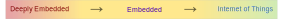
\includegraphics[width=\textwidth]{img/embedded_typen}

    \begin{block}{Beispiele}
        \begin{columns}[onlytextwidth]
            \column[b]{.33\textwidth}
            \includegraphics[width=\textwidth]{img/heart-rate-monitoring-device-1903997_640}

            \column[b]{.33\textwidth}
            \includegraphics[width=\textwidth]{img/blitzer_pulverhausstrasse}

            \column[b]{.33\textwidth}
            \includegraphics[width=\textwidth]{img/winter-681175_640}
        \end{columns}
    \end{block}
\end{frame}
}

%%% Folie
{
\scriptsize

\begin{frame}{Beispiele für typische Single Board Computer}
    \begin{columns}
        \begin{column}[b]{.5\textwidth}
            \textbf{Arduino Nano} \\
            \smallskip
            \includegraphics[width=.5\textwidth]{img/sbc-arduino_nano}

            \begin{itemize}
                \setlength{\itemindent}{-1em}
                \setlength\itemsep{0em}
                \item 16 MHz ATmega328 CPU
                \item 32 KiB Flash EEPROM, 2 KiB SRAM
                \item 22 $\times$ Digital-, 8 $\times$ Analog-, 6 $\times$ PWM-Ausgang
            \end{itemize}
        \end{column}

        \begin{column}[b]{.5\textwidth}
            \textbf{PyBoard} \\
            \smallskip
            \includegraphics[width=.5\textwidth]{img/sbc-pyboard}

            \begin{itemize}
                \setlength{\itemindent}{-1em}
                \setlength\itemsep{0em}
                \item 168 MHz ARM Cortex M4 CPU
                \item 1024 KiB Flash ROM, 192 KiB RAM
                \item 29 GPIO, 3 $\times$ 12-bit ADC, 2 $\times$ 12-bit DAC
            \end{itemize}
        \end{column}
    \end{columns}

    \bigskip

    \begin{columns}
        \begin{column}[b]{.5\textwidth}
            \textbf{ESP32} \\
            \smallskip
            \includegraphics[width=.5\textwidth]{img/sbc-esp32}

            \begin{itemize}
                \setlength{\itemindent}{-1em}
                \setlength\itemsep{0em}
                \item 160 -- 240 MHz Xtensa LX6 Dual-Core CPU
                \item 2 $\times$ 160 KiB RAM (statisch/dynamisch)
                \item GPIO, WLAN, Bluetooth, ...
            \end{itemize}
        \end{column}

        \begin{column}[b]{.5\textwidth}
            \textbf{Raspberry Pi 4} \\
            \smallskip
            \includegraphics[width=.5\textwidth]{img/sbc-raspberrypi}

            \begin{itemize}
                \setlength{\itemindent}{-1em}
                \setlength\itemsep{0em}
                \item BCM2711 ARM v8 CPU, Quad Core
                \item 4 oder 8 GiB RAM
                \item GPIO, WLAN, Bluetooth, USB, HDMI, ...
            \end{itemize}
        \end{column}
    \end{columns}
\end{frame}
}

%%% Folie
{
\scriptsize

\begin{frame}{Mikroprozessoren für eingebettete Systeme}
    \begin{columns}
        \column{.2\textwidth}
        \includegraphics[width=.9\linewidth]{img/chip-intel-486}

        \column{.8\textwidth}
        \begin{block}{Diskreter Hauptprozessor}
            \Justified{
                \smallskip

                Bildet das Herzstück eines jeden Computers bzw. stellt den Computer
                im engeren Sinne dar, basierend auf dem Prinzip
                \textbf{Eingabe-Verarbeitung-Ausgabe}. Kommuniziert daher über eine
                \textbf{Speicherschnittstelle} bestehend aus Adress-, Daten- und Steuerleitungen
                mit externen Speicher- und I/O-Bausteinen.
            }

            \smallskip

            \textbf{Beispiele}: Intel 8051, MOS 6502, Motorola 68000, …
        \end{block}
    \end{columns}

    \begin{columns}
        \column{.2\textwidth}
        \includegraphics[width=.9\linewidth]{img/chip-avr-atmega}

        \column{.8\textwidth}
        \begin{block}{Microcontroller}
            \Justified{
                \smallskip

                Integriert eine einfache CPU (oftmals mit nur 8-bit Datenbreite)
                sowie RAM und ROM auf einem Chip, um ein kleines Programm zur
                Steuerung mit externer Peripherie auszuführen. Bietet meist keine
                externe Speicherschnittstelle, dafür aber I/O-Möglichkeiten wie
                \textbf{GPIO}, \textbf{Serielle Schnittstellen}, \textbf{A/D-Wandler}
                uwm.
            }

            \smallskip

            \textbf{Beispiele}: AVR ATtiny, AVR ATmega, PIC, ARM STM32F722, …
        \end{block}
    \end{columns}

    \begin{columns}
        \column{.2\textwidth}
        \includegraphics[width=.9\linewidth]{img/chip-arm-cortex}

        \column{.8\textwidth}
        \begin{block}{System-on-a-Chip}
            \Justified{
                \smallskip

                Wie ein Microcontroller nur mit einem \textbf{viel leistungsstärkeren
                Rechenkern}, dessen Performance mit dedizierten CPUs vergleichbar ist.
                \textbf{Externer RAM und ROM} werden wie bei einer diskreten CPU über
                ein Speicherinterface angebunden. Darüber hinaus werden oft auch
                \textbf{komplexe Komponenten} wie GPUs, WiFi, Bluetooth, HDMI, etc.
                auf demselben Chip untergebracht.
            }

            \smallskip

            \textbf{Beispiele}: ARM Cortex, AMD AU1000, …
        \end{block}
    \end{columns}
\end{frame}
}

%%% Folie
{
\footnotesize

\begin{frame}{Typischer Systemaufbau eingebetteter Systeme}
    \begin{columns}
        \column{\dimexpr\paperwidth}
        \includegraphics[width=\paperwidth]{img/mc_aufbau}
    \end{columns}

    \bigskip

    \begin{columns}
        \begin{column}[T]{.5\textwidth}
            \textbf{Durchschnittlicher Microcontroller}
            \begin{itemize}
                \item 16 MHz Taktgeschwindigkeit
                \item 8 Bit Wortbreite
                \item 32 kB Programmspeicher
                \item 2 kB Hauptspeicher
                \item 14 General Purpose I/Os
                \item Kein Betriebssystem
            \end{itemize}
        \end{column}
        \begin{column}[T]{.5\textwidth}
            \textbf{Durchschnittlicher System-on-a-Chip}
            \begin{itemize}
                \item $\geq$ 200 MHz Taktgeschwindigkeit
                \item $\geq$ 32 Bit Wortbreite
                \item $\geq$ 512 MB Flash ROM
                \item $\geq$ 16 MB Hauptspeicher
                \item $\geq$ 30 General Purpose I/Os
                \item Mit oder ohne Betriebssystem
            \end{itemize}
        \end{column}
    \end{columns}
\end{frame}
}

%%% Folie
{
\scriptsize

\begin{frame}{Fallbeispiel: Die erste Mondlandung}
    \begin{columns}
        \column{\dimexpr\paperwidth}
        \vskip -.8em
        \includegraphics[width=\textwidth]{img/apollo}
    \end{columns}

    \vskip .5em

    \begin{columns}
        \column{\dimexpr\paperwidth-2em}
        \Justified{
            \textbf{21. Juli 1969}: Apollo 11 bringt die ersten Menschen zum Mond und
            wieder zur Erde zurück. Möglich wird dies unter Anderem durch den ,,Launch
            Vehicle Digital Computer'' der Saturn\,V Rakete und den ,,Apollo Guidance
            Computer'' in der Kommandokapsel.
        }
    \end{columns}
\end{frame}
}

%-------------------------------------------------------------------------------
\section{Erste Schritte mit Python}
%-------------------------------------------------------------------------------

%%% Folie
\begin{frame}{ChatGPT über Python und Java}
    \begin{center}
        \includegraphics[width=.85\textwidth]{img/chatgpt-python-java}
    \end{center}
\end{frame}

%%% Folie
\begin{frame}[allowframebreaks]{ChatGPT über Duck Typing}
    \begin{center}
        \includegraphics[width=.9\textwidth]{img/chatgpt-ducktyping1}
    \end{center}

    %%%
    \framebreak

    \begin{center}
        \includegraphics[width=.9\textwidth]{img/chatgpt-ducktyping2}
    \end{center}

    \begin{center}
        \includegraphics[width=.24\textwidth]{img/duck-typing1}
        \hfill
        \includegraphics[width=.24\textwidth]{img/duck-typing2}
        \hfill
        \includegraphics[width=.24\textwidth]{img/duck-typing3}
        \hfill
        \includegraphics[width=.24\textwidth]{img/duck-typing4}
    \end{center}
\end{frame}

%%% Folie
{
\footnotesize
\setlength{\fboxsep}{0pt}

\begin{frame}{Hilfreiche Webseiten über Python}
    \begin{columns}
        \column[T]{.33\textwidth}
        \fbox{\includegraphics[width=\textwidth]{img/webseite-python}}
        \vskip .5em
        \textbf{Webseite von Python} \\
        \href{https://www.python.org/}{python.org}

        \column[T]{.33\textwidth}
        \fbox{\includegraphics[width=\textwidth]{img/webseite-docs}}
        \vskip .5em
        \textbf{Offizielle Dokumentation} \\
        \href{https://docs.python.org/}{docs.python.org}

        \column[T]{.33\textwidth}
        \fbox{\includegraphics[width=\textwidth]{img/webseite-pypi}}
        \vskip .5em
        \textbf{Python Package Index} \\
        \href{https://pypi.org/}{pypi.org}
    \end{columns}

    \vskip 0.6cm

    \begin{columns}
        \column[T]{.33\textwidth}
        \fbox{\includegraphics[width=\textwidth]{img/webseite-tuten}}
        \vskip .5em
        \textbf{Englisches Tutorial} \\
        \href{https://docs.python.org/3/tutorial/}{docs.python.org/3/tutorial/}

        \column[T]{.33\textwidth}
        \fbox{\includegraphics[width=\textwidth]{img/webseite-tutde}}
        \vskip .5em
        \textbf{Deutsches Tutorial} \\
        \href{https://py-tutorial-de.readthedocs.io/}{py-tutorial-de.readthedocs.io}

        \column[T]{.33\textwidth}
        \fbox{\includegraphics[width=\textwidth]{img/webseite-realpython}}
        \vskip .5em
        \textbf{Real Python} \\
        \href{https://realpython.com/}{realpython.com}
    \end{columns}
\end{frame}
}

%%% Folie
{
\scriptsize

\begin{frame}{Einfache Versuche im Interpreter}
    \begin{columns}
        \column[T]{.7\textwidth}
        \includegraphics[width=\textwidth]{img/python-interpreter-idle}

        \includegraphics[width=\textwidth]{img/python-interpreter-ipython}

        \column[T]{.3\textwidth}
        \Justified{
            Für einfache Versuche oder kleine Wegwerfskripte bietet Python einen
            einfachen Kommandozeileninterpreter, der jede eingegebene Codezeile
            direkt ausführt und ihr Ergebnis ausgibt. Das Prinzip wird auch REPL
            genannt von \textit{Read, Evaluate, Print, Loop}.
            \smallskip

            Traditionell wird der Interpreter, wie im unteren Bild gezeigt, mit dem
            Befehl \texttt{python} in einem Konsolenfenster gestartet. Wobei hier
            die verbesserte Version \texttt{ipython} (separat zu installieren)
            gezeigt wird.
            \smallskip

            Alternativ kann aber auch die im Lieferumfang von Python enthaltene
            grafische Anwendung IDLE gestartet werden.
        }
    \end{columns}
\end{frame}
}

%%% Folie
{
\scriptsize

\begin{frame}{Aufbau eines typischen Python-Projekts}
    \includegraphics[width=\textwidth]{img/verzeichnisse-venv}
    \smallskip

    \Justified{
        Python schreibt im Grunde genommen keine feste Verzeichnisstruktur für ein
        Projekt vor. Dennoch folgen die meisten Projekte den folgenden Konventionen:
    }

    \begin{itemize}
        \item Im Hauptverzeichnis liegen nur ein README und allgemeine Konfigurationsdateien.
        \item Der eigentliche Quellcode des liegt in einem Unterverzeichnis.
        \item Dieses wird durch eine Datei namens \texttt{\_\_init\_\_.py} als Python-Modul gekennzeichnet.
        \item Weitere Verzeichnisse können Dokumentationen und sonstige Zusatzdaten beinhalten.
        \item Benötigte Zusatzbibliotheken werden in die Datei \texttt{requirements.txt} eingetragen.
        \item Die Installation der Bibliotheken erfolgt in einer virtuellen Python-Umgebung.
    \end{itemize}
\end{frame}
}

%%% Folie
{
\tiny

\begin{frame}[fragile]{Virtuelle Python-Umgebungen verwalten}
    \includegraphics[width=\textwidth]{img/env-aktivieren}

    \Justified{
        \medskip
        Python bot schon früh die Möglichkeit, zusätzliche Codebibliotheken aus dem Internet zu laden
        und auf dem eigenen Rechner zu installieren. Traditionell werden die Bibliotheken allerdings
        systemweit installiert, so dass alle Python-Programme dieselben Bibliotheken nutzen. Da aber
        nicht alle Bibliotheken zusammenpassen oder manche Programm unterschiedliche Versionen einer
        Bibliothek verwenden können, kann dies schnell zu Konflikten führen.
        \medskip

        Python ermöglicht es daher, in einem Unterverzeichnis eine isolierte Python-Umgebung für ein
        einzelnes Projekt zu erstellen. Der exakte Inhalt des Verzeichnisses ist für die praktische
        Nutzung dabei gar nicht relevant. Nur, dass dort die Bibliotheken exakt eines Projekts getrennt von
        den anderen Projekten installiert werden. Folgende Kommandozeilenbefehle werden hierfür benötigt:
        \medskip
    }

    {
    %~ \tiny
    \arrayrulecolor{gray}

    \begin{tabular}{|p{.95\textwidth}|}
        \hline

        \cellcolor{gray!15}
        \texttt{python -m venv env} \\
        \cellcolor{gray!15}
        \textcolor{darkgray}{Neue Pythonumgebung im Verzeichnis \texttt{env} anlegen} \\

        \cellcolor{gray!7}
        \\

        \cellcolor{gray!15}
        \texttt{source env/bin/activate} bzw. \\
        \texttt{. env/bin/activate} \\
        \cellcolor{gray!15}
        \textcolor{darkgray}{\textbf{Linux, Mac:} Python-Umgebung für die laufende Konsolensitzung aktivieren} \\

        \cellcolor{gray!7}
        \\

        \cellcolor{gray!15}
        \texttt{env\textbackslash Scripts\textbackslash activate} \\
        \cellcolor{gray!15}
        \textcolor{darkgray}{\textbf{Windows:} Python-Umgebung für die laufende Konsolensitzung aktivieren} \\

        \cellcolor{gray!7}
        \\

        \cellcolor{gray!15}
        \texttt{deactivate} \\
        \cellcolor{gray!15}
        \textcolor{darkgray}{Aktuelle aktive Python-Umgebung wieder verlassen} \\

        \hline
    \end{tabular}
    }

    \medskip
    \LinkButton{https://realpython.com/python-virtual-environments-a-primer/}{Ausführliche Anleitung}
\end{frame}

%%% Folie
{
\scriptsize

\begin{frame}{Probleme mit der PowerShell unter Windows}
    \Justified{
        Die Sicherheitseinstellungen von Windows verbieten normalerweise die
        Ausführung von PowerShell-Skripten. Dies dient als Vorsorge gegen
        Skript-Viren, die bis in die frühen 2000er-Jahre ein großes Problem
        darstellten. Dadurch bricht die Aktivierung eines Python-Environments
        allerdings mit einer Fehlermeldung ab.
    }

    \begin{center}
        \includegraphics[width=.8\textwidth]{img/powershell1}
    \end{center}

    \Justified{
        Um die entsprechende Einstellung zu ändern, muss die PowerShell einmal
        als Administrator geöffnet werden. Folgender Befehle fragen die Einstellung
        ab, bzw. ändern sie:
        \smallskip

        \texttt{Get-ExecutionPolicy} \\
        \texttt{Set-ExecutionPolicy RemoteSigned -Scope CurrentUser}
    }

    \begin{center}
        \includegraphics[width=.8\textwidth]{img/powershell2}
    \end{center}

    \LinkButton{https://learn.microsoft.com/en-us/powershell/module/microsoft.powershell.security/set-executionpolicy?view=powershell-7.3}{Dokumentation von Microsoft}
\end{frame}
}

%%% Folie
{
\tiny

\begin{frame}[fragile]{Abhängigkeiten installieren mit pip}
    \includegraphics[width=\textwidth]{img/pip-install}

    \includegraphics[width=\textwidth]{img/pip-list}

    \Justified{
        \medskip
        Die Installation und Deinstallation der Bibliotheken erfolgt mit dem Kommandozeilenwerkzeug
        \texttt{pip} durch Ausführen der unten aufgeführten Befehle. Dabei hat es sich als Best-Practice
        etabliert, die Bibliotheken und ihre Versionen in einer Datei namens \texttt{requirements.txt}
        zu beschreiben, damit die Installation jederzeit reproduziert werden kann:
    }

    \begin{lstlisting}[language=Python, gobble=8]
        # Farbige und formatierte Konsolenausgaben
        rich~=13.2
    \end{lstlisting}

    {
    %~ \tiny
    \arrayrulecolor{gray}

    \begin{tabular}{|p{.95\textwidth}|}
        \hline

        \cellcolor{gray!15}
        \texttt{pip install -r requirements.txt} \\
        \cellcolor{gray!15}
        \textcolor{darkgray}{Alle in der angegebenen Datei aufgezählten Bibliotheken installieren} \\

        \cellcolor{gray!7}
        \\

        \cellcolor{gray!15}
        \texttt{pip install \textit{bibliothek}} \\
        \cellcolor{gray!15}
        \textcolor{darkgray}{Manuelle Installation einer einzelnen Bibliothek (nicht empfohlen!)} \\

        \cellcolor{gray!7}
        \\

        \cellcolor{gray!15}
        \texttt{pip uninstall \textit{bibliothek}} \\
        \cellcolor{gray!15}
        \textcolor{darkgray}{Manuelle Deinstallation einer einzelnen Bibliothek (nicht empfohlen!)} \\

        \cellcolor{gray!7}
        \\

        \cellcolor{gray!15}
        \texttt{pip list} \\
        \cellcolor{gray!15}
        \textcolor{darkgray}{Bereits installierte Bibliotheken und ihre Version auflisten} \\

        \hline
    \end{tabular}
    }
\end{frame}
}

%%% Folie
{
\tiny

\begin{frame}[fragile]{Verwendung der Bibliothek und Start der Anwendung}
    \Justified{
        Bei aktivierter virtueller Python-Umgebung kann die Anwendung wie folgt gestartet werden.
        Die hier verwendete Bibliothek \texttt{rich} wurde zuvor dem Projekt hinzugefügt.
    }

    \includegraphics[width=\textwidth]{img/venv-ausfuehren}

    \begin{lstlisting}[language=Python, gobble=8]
        #! /usr/bin/env python
        """
        Minimalbeispiel für ein typisches Python-Projekt.
        """

        import rich
        from rich.prompt import Prompt

        if __name__ == "__main__":
            name = Prompt.ask(
                "[bold bright_magenta]Wie heißt du?[/bold bright_magenta]",
                default="Kain Ame"
            )

            eis = Prompt.ask(
                "[bold bright_magenta]Welches ist dein Lieblingseis?[/bold bright_magenta]",
                choices = ["Schokolade", "Vanille", "Erdbeer"],
                default = "Erdbeer"
            )

            rich.print(f"Hallo, [red]{name}[/red]. Dein Lieblingseis ist [blue]{eis}[/blue]. :red_heart-emoji:\n")
    \end{lstlisting}
\end{frame}
}

%%% Folie
{
\tiny

\begin{frame}{Poetry als moderne Alternative}
    \includegraphics[width=\textwidth]{img/verzeichnisse-poetry}
    \smallskip

    \Justified{
        Für Umsteiger von anderen Programmiersprachen wie zum Beispiel JavaScript/Node.js scheint
        die manuelle Verwaltung virtueller Python-Umgebungen sicher etwas umständlich. In den letzten
        Jahren sind deshalb viele Werkzeuge zur Automatisierung und Vereinfachung wie Poetry erschienen.
        Die Konventionen für die Verzeichnisstruktur sind nahezu dieselben wie bei den älteren Werkzeugen.
        Jedoch entfällt hier das Verzeichnis für die virtuelle Umgebung, da dieses von Poetry automatisch
        außerhalb des Projektverzeichnisses angelegt wird:
    }

    \begin{itemize}
        \item Im Hauptverzeichnis liegen nur ein README und allgemeine Konfigurationsdateien.
        \item Der eigentliche Quellcode des liegt in einem Unterverzeichnis.
        \item Dieses wird durch eine Datei namens \texttt{\_\_init\_\_.py} als Python-Modul gekennzeichnet.
        \item Weitere Verzeichnisse können Dokumentationen und sonstige Zusatzdaten beinhalten.
    \end{itemize}

    \Justified{
        Ebenfalls neu ist die Datei \texttt{pyproject.toml}, welche die \texttt{requirements.txt}
        ersetzt. Sie enthält neben den benötigten Bibliotheken noch weitere Einstellungen für
        das Projekt. Die Datei \texttt{poetry.lock} stellt sicher, das bei einer Wiederholung der
        Installation die exakt gleichen Versionen aller Bibliotheken installiert werden.
        \smallskip
    }

    \LinkButton{https://python-poetry.org/}{Poetry Paketverwaltung}
\end{frame}
}

%%% Folie
{
\tiny

\begin{frame}[fragile]{Wichtige Befehle für Poetry}
    \includegraphics[width=\textwidth]{img/poetry-show}

    \Justified{
        \medskip
        Alle für die Arbeit an einem Projekt relevanten Aufgaben können mit dem \texttt{poetry}
        Kommandozeilenwerkzeug erledigt werden. Eine Unterscheidung, ob eine virtuelle Python-Umgebung
        verwaltet oder Bibliotheken darin installiert werden sollen, gibt es nicht. Peoptry kümmert
        sich im Hintergrund selbstständig darum, eine virtuelle Umgebung für das Projekt anzulegen
        und zu verwalten.
        \medskip
    }

    {
    %~ \tiny
    \arrayrulecolor{gray}

    \begin{tabular}{|p{.95\textwidth}|}
        \hline

        \cellcolor{gray!15}
        \texttt{poetry init} \\
        \cellcolor{gray!15}
        \textcolor{darkgray}{Anlegen eines neuen Python-Projekts} \\

        \cellcolor{gray!7}
        \\

        \cellcolor{gray!15}
        \texttt{poetry install} \\
        \cellcolor{gray!15}
        \textcolor{darkgray}{Erzeugen der Python-Umgebung und Installation aller bekannten Abhängigkeiten} \\

        \cellcolor{gray!7}
        \\

        \cellcolor{gray!15}
        \texttt{poetry add \textit{bibliothek}} \\
        \cellcolor{gray!15}
        \textcolor{darkgray}{Installieren und Hinzufügen einer weiteren Bibliothek zum aktuellen Projekt} \\

        \cellcolor{gray!7}
        \\

        \cellcolor{gray!15}
        \texttt{poetry remove \textit{bibliothek}} \\
        \cellcolor{gray!15}
        \textcolor{darkgray}{Deinstallieren und Entfernen einer Bibliothek aus dem aktuellen Projekt} \\

        \cellcolor{gray!7}
        \\

        \cellcolor{gray!15}
        \texttt{poetry show} \\
        \cellcolor{gray!15}
        \textcolor{darkgray}{Informationen zu allen installierten Bibliotheken anzeigen} \\

        \cellcolor{gray!7}
        \\

        \cellcolor{gray!15}
        \texttt{poetry run \textit{befehl}} \\
        \cellcolor{gray!15}
        \textcolor{darkgray}{Ausführen des übergebenen Kommandozielenbefehls innerhalb der Python-Umgebung} \\

        \cellcolor{gray!7}
        \\

        \cellcolor{gray!15}
        \texttt{poetry shell} \\
        \cellcolor{gray!15}
        \textcolor{darkgray}{Start einer Sub-Shell mit aktivierter, virtueller Pyhton-Umgebung} \\

        \cellcolor{gray!7}
        \\

        \cellcolor{gray!15}
        \texttt{poetry shell} \\
        \cellcolor{gray!15}
        \textcolor{darkgray}{Verlassen der Sub-Shell und somit der virtuellen Python-Umgebung} \\

        \hline
    \end{tabular}
    }
\end{frame}
}

%%% Folie
{
\tiny

\begin{frame}[fragile]{Start eines Poetry-Projekts}
    \includegraphics[width=\textwidth]{img/poetry-run1}

    \includegraphics[width=\textwidth]{img/poetry-run2}

    \Justified{
        \medskip
        Mit dem Kommando \texttt{poetry run \textit{befehl}} lässt sich die virtuelle Python-Umgebung
        temporär für die Ausführung das angegebenen Betriebssystembefehls aktivieren. Meistens wird
        dies einfach nur genutzt, um die Anwendung wie oben gezeigt zu starten. Es kann aber auch eine
        IDE wie Visual Studio Code somit gestartet werden, um ein Debuggen der Anwendung darin zu
        ermöglichen:
    }

    \begin{lstlisting}[language=sh, gobble=8]
        poetry run code
    \end{lstlisting}

    \includegraphics[width=\textwidth]{img/poetry-vscode}
\end{frame}
}

% Code und Screenshot

%-------------------------------------------------------------------------------
\section{Remote-Entwicklung mit VS Code}
%-------------------------------------------------------------------------------

%%% Folien
{
\scriptsize
\setlength{\fboxsep}{0pt}

\begin{frame}[allowframebreaks]{Testen der SSH-Verbindung}
    \begin{center}
        \fbox{\includegraphics[width=\textwidth]{img/ssh-ip-addr-show}}
    \end{center}

    \Justified{
        Mit dem Befehl \texttt{ip -brief addr show} lassen sich die IP-Adressen des Raspberry Pi anzeigen.
        Diese werden für den Remote-Login mit SSH benötigt, um den Raspberry Pi auch ohne Bildschirm,
        Tastatur und Maus programmieren vom Laptop aus programmieren zu können.
    }

    %%%
    \framebreak

    \begin{center}
        \fbox{\includegraphics[width=\textwidth]{img/ssh-erstlogon}}
    \end{center}

    \Justified{
        Auf dem eigenen Laptop kann der Logon mit folgendem Befehl getestet werden:
        \smallskip

        \texttt{ssh \textit{benutzername}@\textit{ip-adresse}}
        \smallskip

        Es sollten eine einmalige Sicherheitsabfrage sowie der Login-Prompt des Raspberry Pi
        erscheinen. An diesem sollte man sich mit dem während der Installation angelegten
        Benutzerkonto anmelden können. Mit dem Befehl \texttt{exit} kann die Anmeldung
        danach beendet werden.
        \smallskip

        \textcolor{MidnightBlue}{
            Da sich die IP-Adresse jederzeit ändern kann, werden wir demnächst das Werkzeug
            \textbf{find-my-device} auf dem Raspberry Pi installieren. Damit lässt sich die
            IP-Adresse dann ganz einfach durch Aufrufen einer Webseite ermitteln. Das Werkzeug
            programmiere ich gerade. \smiley{}
            \smallskip
        }

        \textcolor{darkred}{
            Zum Ausschalten führen Sie den Befehl \texttt{sudo poweroff} aus, bevor Sie den
            Strom trennen. EIn hartes Ausschalten ohne diesen Befehl ist nur erlaubt, wenn
            das Dateisystem read-only eingehängt wurde, um Datenverluste zu vermeiden!
        }
    }
\end{frame}
}

%%%%%%%
% TODO: Folien zu "Find my Device"
%%%%%%%

%%% Folien
{
\scriptsize
\setlength{\fboxsep}{0pt}

\begin{frame}[allowframebreaks, fragile]{Remote-Verbindung herstellen}
    \begin{columns}
        \column[c]{.6\textwidth}
        \fbox{\includegraphics[width=\textwidth]{img/vscode-01}}

        \fbox{\includegraphics[width=\textwidth]{img/vscode-02}}

        \fbox{\includegraphics[width=\textwidth]{img/vscode-03}}

        \column[c]{.4\textwidth}
        \Justified{
            Zunächst muss eine neue SSH-Verbindung angelegt werden:
        }

        \begin{enumerate}
            \item Kommandopalette öffnen mit \texttt{Shift+Strg+P}
            \item Nach ,,Remote-SSH'' suchen
            \item Den Eintrag ,,Connect Current Window To Host...'' auswählen
            \item Für die Verbundungsdaten \texttt{\textit{benutzername}@\textit{ip-adresse}} eingeben
        \end{enumerate}
    \end{columns}

    %%%
    \framebreak

    \begin{columns}
        \column[c]{.6\textwidth}
        \fbox{\includegraphics[width=\textwidth]{img/vscode-01}}

        \fbox{\includegraphics[width=\textwidth]{img/vscode-04}}

        \fbox{\includegraphics[width=\textwidth]{img/vscode-05}}

        \fbox{\includegraphics[width=\textwidth]{img/vscode-06}}

        \column[c]{.4\textwidth}
        \Justified{
            Anschließend kann die eben angelegte Verbindung hergestellt werden:
        }

        \begin{enumerate}
            \item Kommandopalette öffnen mit \texttt{Shift+Strg+P}
            \item Erneut nach ,,Remote-SSH'' suchen und ,,Connect Current Window To Host...'' auswählen
            \item Die eben angelegte Verbindung anklicken
            \item Auf Nachfrage das Benutzerpasswort eingeben
            \item Abwarten, bis der Workspace auf dem Raspberry Pi eingerichtet wurde
        \end{enumerate}
    \end{columns}
\end{frame}
}

%%% Folien
{
\scriptsize
\setlength{\fboxsep}{0pt}

\begin{frame}[allowframebreaks, fragile]{Fallbeispiel: Hallo, Raspberry Pi}
    \begin{center}
        \fbox{\includegraphics[width=.9\textwidth]{img/vscode-07}}
    \end{center}

    \Justified{
        Mit \texttt{Strg+Ö} (wie englisch ,,Törminal'' \smiley{}) kann eine Konsole geöffnet werden,
        um Befehle auf dem Raspberry Pi auszuführen. Der Befehl \texttt{mkdir \textit{verzeichnis}}
        legt ein neues Quellcodeverzeichnis an, das anschließen über den Button ,,Open Folder''
        im linken Bereich geöffnet werden kann.
    }

    %%%
    \framebreak

    \begin{columns}
        \column[c]{.6\textwidth}
        %~ \fbox{\includegraphics[width=\textwidth]{img/vscode-08}}

        \fbox{\includegraphics[width=\textwidth]{img/vscode-09}}

        \fbox{\includegraphics[width=\textwidth]{img/vscode-10}}

        \column[c]{.4\textwidth}
        \Justified{
            Weil das verzeichnis noch leer ist, werden links noch keine Dateien angezeigt.
            Mit Rechtsklick soll daher eine Datei namens \texttt{main.py} angelegt werden.
            \smallskip

            Die Frage, ob die empfohlenen Erweiterungen für die Pythonprogrammierung in
            Visual Studio Code installiert werden sollen, kann mit Klick auf ,,Install''
            bestätigt werden. Die Erweiterungen vereinfachen ein wenig das Programmieren
            durch Codeverschläge und Prüfungen.
        }
    \end{columns}

    %%%
    \framebreak

    \begin{columns}
        \column[c]{.54\textwidth}
        %~ \fbox{\includegraphics[width=\textwidth]{img/vscode-11}}

        \fbox{\includegraphics[width=\textwidth]{img/vscode-12}}

        \fbox{\includegraphics[width=\textwidth]{img/vscode-13}}

        \column[c]{.45\textwidth}
        \Justified{
            Die Datei soll folgenden Inhalt besitzen:
        }

        \begin{lstlisting}[language=Python, gobble=12]
            def main():
                name = ""

                while not name:
                    name = input("Wie heißt du? ")

                print(f"Hallo, {name}!")

            if __name__ == "__main__":
                try:
                    main()
                except KeyboardInterrupt:
                    pass
        \end{lstlisting}

        \bigskip

        \Justified{
            Über den Eintrag ,,Run Python File in Terminal'' im Kontextmenü (Rechtsklick)
            lässt sich das Programm ausführen. Das Ergebnis sollte wie im unteren Screenshot
            aussehen.
        }
    \end{columns}
\end{frame}
}
